% Thesis!

% Two Column Format
\documentclass[11pt]{article}
%this allows us to specify sections to be single or multi column so that things like title page and table of contents are single column
\usepackage{multicol, caption}
\usepackage{verbatim}
\usepackage{listings}
\usepackage{color}
\usepackage{todonotes}

\definecolor{dkgreen}{rgb}{0,0.6,0}
\definecolor{gray}{rgb}{0.5,0.5,0.5}
\definecolor{mauve}{rgb}{0.58,0,0.82}

\lstdefinelanguage{JavaScript}{
  keywords={typeof, new, true, false, catch, function, return, null, catch, switch, var, if, in, while, do, else, case, break},
  keywordstyle=\color{blue}\bfseries,
  ndkeywords={class, export, boolean, throw, implements, import, this},
  ndkeywordstyle=\color{darkgray}\bfseries,
  identifierstyle=\color{black},
  sensitive=false,
  comment=[l]{//},
  morecomment=[s]{/*}{*/},
  commentstyle=\color{purple}\ttfamily,
  stringstyle=\color{red}\ttfamily,
  morestring=[b]',
  morestring=[b]"
}

\lstset{frame=tb,
  language=JavaScript,
  aboveskip=3mm,
  belowskip=3mm,
  showstringspaces=false,
  columns=flexible,
  basicstyle={\small\ttfamily},
  numbers=none,
  numberstyle=\tiny\color{gray},
  keywordstyle=\color{blue},
  commentstyle=\color{dkgreen},
  stringstyle=\color{mauve},
  breaklines=true,
  breakatwhitespace=true
  tabsize=3
}

\usepackage{setspace}
\usepackage{url}

\usepackage{graphicx}

%%% PAGE DIMENSIONS
\usepackage{geometry} % to change the page dimensions
\geometry{letterpaper}

\setcounter{secnumdepth}{5}

\graphicspath{ {./images/} }

\newenvironment{Figure}
  {\par\medskip\noindent\minipage{\linewidth}}
  {\endminipage\par\medskip}

\begin{document}

%%%%%%%%%%%%%%%%%%
%%% Cover Page %%%
%%%%%%%%%%%%%%%%%%

\title{\vfill A Survey of Web Testing Frameworks and a Workflow for Testing Javascript Applications} %\vfill gives us the black space at the top of the page
\author{
By Taggart Ashby \vspace{10pt} \\
}

\maketitle

\vfill  %in combination with \newpage this forces the abstract to the bottom of the page

%%%%%%%%%%%%%%%%
%%% Abstract 
%%% VERY General overview of problem and solution in paper
%%%%%%%%%%%%%%%%
\begin{abstract}
\todo{Make this better}
Web applications are quickly replacing standalone applications. As with any type of applicaiton, these web applications need to be tested to ensure proper functionality and reliability. There have been substantial efforts to create tools to help with the testing of web applicaitons but there is, as of yet, no standard or recommended workflow to insure speed of development and strength of application.

We have brought together a number of testing tools from the web and created what we feel is a fully-featured, easy to use, testing framework and workflow for javascript web applications.
\end{abstract}

\thispagestyle{empty} %remove page number from title page
\newpage

%end the 1 column format

%start 2 column format
% \begin{multicols}{2}
%Start numbering first page of content as page 1
\setcounter{page}{1}

%%%%%%%%%%%%%%%%%%%%
%%% Introduction/Motivation
%%% More detailed, but still general, description of problem and why we want to solve it
%%%%%%%%%%%%%%%%%%%%
\section{Introduction}
Since the advent of the internet, the web has undergone an impressive evolution from plain-text webpages to the highly stylized and functional pages that we see today. In the last four to six years there has been an explosion of new web technologies that make applications more functional: HTML5, CSS3, WebGL, Touch APIs, Geo-location, and a host of others. \cite{EvolutionOfWeb} In that same time period, the number of global internet users has grown to somewhere around 2.5 billion people. \cite{EvolutionOfWeb} The combination of these new technologies and the ever-increasing usage of the internet has led to a significant growth in the number and complexity of web applications.

Like any piece of software, these web applications require testing in order to determine their correctness and give their users the best experience possible. Unfortunately, web applications are new and there are no standard practices regarding how to test them. Their dynamic nature and network communication require a different testing toolkit than their predecessors. In addition, web applications are being produced at an incredible rate and so there's a need for rapid testing.

We can see that this is not a solved problem by looking at some of the biggest web application around. A 2011 study showed that YouTube has at least eight errors, Apple has at least seven, Microsoft at least four, and the list goes on. \cite{ErrorsInTheWild} That may seem like a incredibly small amount for such monoliths, and, honestly, it is fairly small, but those are still errors in the software that ought to be fixed.

What this all boils down to is that there needs to be a framework in place for testing these multi-layer, multi-faceted web applications that is easy to use, quick to develop on, and thorough in its coverage.

\subsection{What Has Been Done Already?}
Web developers are not clueless, they understand that there is a need for testing of web applications. Unfortunately, web development is still a relatively new domain and developers have not come together to work on the problem of testing but rather have come up with their own proprietary solutions in isolation or merely on a per-project basis. Some of these tools have gained traction and become larger, more general, tools.

\todo{What goes here?}
\todo{Info info info}

\subsubsection{Why It Is Insufficient}
% - No standard
The problem that followed was that many of the tools attempted to remedy the same problems and so a developer would have to decide between a number of similar tools. Having to wade through a sea of similar tools is time-consuming and that can be the death of a cutting-edge application. The more time an application is off the market, the more time competitors have to develop their own versions. Yet another problem is that deciding between similar tools can be discouraging to the developer that just wants to write their application and test it quickly.

\todo{Info info info}

\subsection{Problems Still Faced/Why It's So Hard}
% - A lot of products to test against (browsers)
Testing web applications is difficult. The web offers an impressive set of features, but with those features come some draw-backs. Two of the most frustrating drawbacks for developers are the number of platforms and the web's asynchronous nature.

In the very beginning, web applications were easy to write and test because the only code was straight HTML with a common set of HTML tags. It didn't matter what browser was used to view the content because the viewer was always a home computer rendering plain HTML. As time progressed individual browsers began offering additional features and web applications became more rich but harder to test because the developer would need to run their code on a couple different browsers to make sure they all behaved similarly. In today's technological world, it is nearly impossible to run one's web application on all of the possible browser versions, configurations, and platforms that are available. Web applications are on home computers, phones, tablets, MP3 players, refrigerators \cite{SamsungFridge}, and a variety of other devices of varying sizes and capabilities. As a developer, one wants to target as many of those platforms as possible with a single code-base to save oneself time and effort. A naive developer might just release an application on all platforms and hope for the best, but releasing on all platforms without testing will likely drive consumers away if the application fails on their given platform.

% - Asynchronous shennanigans
The addition of Javascript to web applications led to a golden age of feature-rich applications with exciting UI that had not before been seen. This set of features and UI improvements came with an, albeit necessary, complication of asynchronous execution. Unlike traditional multi-threaded software, however, the developer is not given access to individual threads but is stuck with just the main thread. This sort of implementation is essential for dealing with asynchronous events like button clicks, data loading that doesn't hold up the web page, and a variety of other niceties, but is the cause of major headaches in testing. Without access to individual threads, the developer has to either write synchronous code that will be slow and not user-friendly, or rely on other mechanisms that allow code to be sequenced. Often it is hard to get code properly sequenced and it requires changing straightforward functions to a hideous amalgamation of callbacks.

There is no overarching solution to these problems, but in order to understand the motivations behind this thesis, one must understand the problems facing web application developers.

\subsection{Contributions of This Thesis}
%- Framework
The goal of this thesis is to bring together tools that are already available for testing and combine them into a single framework that offers web application developers a toolkit for their testing needs. There are plenty of strong tools available and we hope to gather a subset of those tools to cover as much of the testing spectrum as possible. 

In addition to creating a single framework, we've set out to weigh the options between the most popular frameworks so that a developer need not just blindly trust our recommendations. Since every project is unique, a single set of tools cannot possibly cover the gamut. In addition to the single set of recommendations, the most popular tools are discussed so that the devloper is free to pick and choose as they see fit.
%- Wade through all the tools currently out there
%-- Focus in, no need to have every developer check out all 10000 tools
%-- Weigh options

%%%%%%%%%%%%%%%%%%
%%% Background 
%%% Information needed for reader to know what’s going on
%%% 	Server/Client Communication
%%% 	Cloud services
%%% 	Appropriate terms and definitions
%%%%%%%%%%%%%%%%%%
\section{Background}
In an effort to make the rest of the paper more understandable and to define the terms used in the remainder of the paper, we will outline the various concepts and technologies surrounding the web.
If one is familiar with HTML5, JavaScript, and Testing concepts and statistics, it will likely be safe to skip this background section.

\subsection{Web Application Strengths}
Web applications are great for both developers and consumers. They have a number of characteristics that make them more desirable than shrink-wrap software. These attributes are versioning, availability, platform independence, and the ability to rapidly prototype.

\subsubsection{Versioning}
Web applications can be updated at any time with instant roll-out and feedback. It requires absolutely no user interaction because the web page always serves the latest resources. In comparison to something like an operating system that requires users to manually update, this feature leads to applications that can address problems quickly, roll-out security updates instantly, and incorporate consumer feedback much more quickly than any other type of software. Another perk is that users are not given a choice. This can lead to occasional customer outrage, but more often than not it's a powerful gain for both feature improvement and application security.

\subsubsection{Availability}
Web application are available anywhere there's internet. No need to install anything on a given device most of the time. Due to the ever-increasing popularity of mobile devices, most applications have both mobile and full versions of their software and so the application is ``with'' the user all the time.

\subsubsection{Multi-platform}
Very similar to the availability strength, web applications are platform independent. Whether the user is on their phone, tablet, laptop, or PC, the application only requires a web browser with certain functionality and in this day and age all devices come equipped with browsers that should have no problems.

\subsubsection{Rapid Prototyping}
Web applications are fantastic for rapid prototyping because of all of the strengths discussed above. An idea can be prototyped and posted on a website quickly and rapid iteration can occur without the user even necessarily noticing. There are a number of web tools that will outline where users are clicking, what features they're using, how long they're spending on a given page or step of a process, and a number of other metrics that can make iterations more directed and effective.

\subsection{Web Features}
Here we'll discuss some of the prevalent technologies that recently appeared in web applications and development. By no means is this an exhaustive list, just a sampling of the more prominent ones.

\subsubsection{HTML5}
The latest revision of HTML is HTML5 which first debuted on Firefox back in 2009. \cite{EvolutionOfWeb} HTML5 has not been officially recommended by the W3C (World Wide Web Consortium) who is the official keeper and recommender of web standards, however, there is a plan for final recommendation this year, 2014, called Plan 2014. \cite{Plan2014} What this means is that in 2014 the W3C will release a stable HTML5 Recommendation which will make HTML5 an official standard and help universalize all the separate implementations.

HTML5 brings a number of new features including: audio and video tags, the canvas element, drag-and-drop functionality, web storage, offline page support, and a number of other modern web features. A lot of HTML5's features revolve around the inclusion of multimedia in web pages and stronger graphical processing and programming.

As the web is being increasingly used on mobile devices, HTML5 also introduces geolocation functionality. This funcationality requires user approval, but once that approval is gained, the web application has access to a rough idea of where the user is located. When used on devices that have GPS, such as phones and tablets, this area is more defined and a stronger lock on the user's position can be obtained. This geolocation functionality has opened the door for brand new types of web applications that can much more closely tie in with what the user is seeing or the area that they are in. For example, ads can be more targeted or an application can display distances to nearby points of interest.

JavaScript, though not the only scripting language with web use, is the primary language used to compliment HTML5 when making web applications. It is an interpreted language that is most often associated with client-side functionality, but in recent times has extended to the server-side. JavaScript is a prototype based object oriented scripting language with dynamic typing and first-class functions. Much of JavaScript's popularity stems from this dynamic nature that allows for quick, and often dirty, implementation of features in an iterative environment.

%\todo{THIS NEEDS TO MOVE OR CHANGE SUBSECTION TO `WEB APPLICATIONS'}
\paragraph{Node.JS}
As a quick aside, it will be useful to have information about Node.JS as it is used in the sample application and the evaluation applicaiton. Node.JS, often called simply Node, is a JavaScript API for creating and running servers. ``Node's goal is to provide an easy way to build scalable network programs.'' \cite{Node} Node was created in 2009 and is sponsored by Joyent. Node does not use thread-based networking, instead opting for a single-threaded event loop and non-blocking I/O. Node allows developers to create and control web servers without the need for external software, such as Apache, commonly found in other sites.

Node is found in a number of popular sites including: PayPal, The New York Times, Yahoo!, Uber, LinkedIn, Microsoft Azure, and a number of others. \cite{Node}


\todo{TIE THIS CLIENT/SERVER STUFF into Web Applications, be specific, not generic}
\subsection{Client/Server Architecture}
Web applications have a user-facing client-side and a ``rear-facing'' \todo{IS THIS THE RIGHT TERM...} server-side.

Here we'll discuss what the client-side is and does, what the server-side is and does, and how they communicate.

\subsubsection{What is the Client-side Portion?}
First, we'll address what a client is. The simple answer is: The User. The User's phone, computer, tablet, or other device communicating with a given website or application is the client. More specifically, the browser or service being using to communicate with the web is the client. 

So now that the client has been clarified, what is the client-side portion of an application? The client-side portion interacts with the browser to request assets from the server and then displaying them in a human-readable way. The client-side also deals with the user interface and interactivity of a web page, e.g., the client-side displays a web form, the client fills in the information and clicks ``submit'' and the client-side packages up the data and sends it to the server-side.

Client-side programming is done in a language that the browser understands, most frequently Javascript. Though not technically programming languages, client-side programming is also done through HTML and CSS which control the look and feel of web pages.

\subsubsection{What is the Server-side Portion?}
Once again, we'll outline a server and then delve into server-side programming. A server is the entity, be it machine, person, or cloud service, that stores the information about a given web page or application. The server stores all assets, HTML pages, images, videos, databases, etc, and provides them upon request to the client. The server also handles all of the processing for interactivity, accounts, and a general number-crunching.

The server-side portion of an application, then, stores all of the assets, accounts, and structure of the entire application. The server-side authenticates users, retrieves data from databases, processes large data, and send information, be it assets or results, back to the client to display to the user.

\subsubsection{Client and Server Interactions}
The client has limited access to resources on any given web application. This access is restricted by the server. Without such restrictions in place, someone could access user databases, credit card information, order reports, etc. In addition, there would be an overwhelming amount of content for a client to parse through, even if they have no malicious intent.

Clients communicate with the Server through a request-response architecture. Clients send a request to the server, sometimes with information attached, such as a form submittal or login, and the server returns a response with either a success/failure message, or additional data.


\subsection{What is testing?}
IEEE defines software testing as ``the dynamic verification of the behavior of a program on a finite set of test cases, suitably selected from the usually infinite executions domain, against the expected behavior.'' \cite{TestingDefinition} Put a bit more simply, software testing is the process of making sure the program does what it is supposed to.

There are a number of different types of tests and testing concept, we will just focus on Unit Testing, Continuous Integration, and Acceptance Testing.

\subsubsection{Unit Testing}
Unit testing is the testing of specific functions and functionality, or ``test units.'' Test units are ``A set of one or more computer program modules together with associated control data, [...] usage procedures, and operating procedures taht satisfy the following conditions: 1) All modules are from a single computer program. 2) At least one of the new or changed modules in the set has not completed the unit test. 3) The set of modules together with its associated data and procedures are the sole object of a testing process.'' \cite{UnitTestDefinition} Generally this means the testing of individual functions but can extend to a set of functions that produce a single module of functionality. What sets Unit Testing apart from other types of testing is that tests focus on one portion of the code or system rather than interactions between modules or the entire system.

Here's a brief example:
\begin{lstlisting}
// Terribly useless code whose purpose is to eventually calculate a magic number
function addTwo (numToAddTo) {
	return numToAddTo + 2;
}

function twoTimes (numToMultiply) {
	var sum = 0;

	for (var i = 0; i < numToMultiply; i++) {
		sum = addTwo(sum);
	}

	return sum;
}

.... // More functions

function calculateMagicNumberPartOne (startingNum) {
	var foo = 3 + addTwo(startingNum);

	return twoTimes(foo);
}

... // More functions

function calculateMagicNumber (startingNum) {
	var numSoFar = calculateMagicNumberPartOne(startingNum);

	numSoFar = calculateMagicNumberPartTwo(numSoFar);
	numSoFar = calculateMagicNumberPartThree(numSoFar);
	... // More calculateMagicNumberPart(s)

	return numSoFar;
}

function testAddTwo () ... // Unit Test
function testTwoTimes () ... // Unit Test
function testCalculateMagicNumberPartOne () ... // Still a Unit Test, just a whole module of functionality

function testCalculateMagicNumber () ... // NOT a Unit Test because it's testing the whole system
\end{lstlisting}

Unit tests are important because they are done in isolation from one another. The purpose of a unit test is to ensure that once individual modules are put together, the developer need only focus on the interaction between them instead of their individual functionality. Without the assurances of prior unit tests, integration would be a more stressful and mysterious proposition.

\subsubsection{Continuous Integration}
The original definition of Continuous Integration involves the idea of developers committing from their  branches to a master branch daily so that changes are continuously integrated in an effort to make sure all branches can, in fact, be integrated. It has since evolved into a more general idea of a tool that runs commands after each commit to a repository. This commands generally encompass running unit tests, integration tests, user interface tests, and also often publishing and disseminating notifications to interested parties. This is invaluable feedback because the developer can see if they're making progress in the right direction as they write code, as opposed to a situation in which the developer finishes coding and finds out they've made a bad assumption or decision between this commit and the last. 

One of the most important aspects of a good piece of CI software is that it is automatic. There should be no need for a developer to do anything besides, perhaps, ``turn it on'' and start coding. As soon as a tool, CI or otherwise, requires more than one or two interactions to run, it becomes more of a nuisance and less of an asset.

\subsubsection{Acceptance Testing}
Acceptance testing is testing to confirm that the product meets a certain specification. Often this is making sure that the software meets an SRS (Software Requirements Specification) or a customer's outlined expectations. Often this testing is performed by the user of the software or customer that ordered the software, rather than the developers.

In an effort to automate this, some developers create ``User Stories'' which are automated tests that run a series of functions described by customers or an SRS. These User Stories are often written in a seperate language that is more like english than code. The traditional User Story template is: ``As a <role>, I want <goal/desire> so that <benefit>.'' For example: ``As a supervisor, I want to find my employees by their employee ID.'' These user stories are then broken down into more specific steps that can be automated.

\subsubsection{Testing Statistics}
It is widely accepted that the earlier a developer detects a defect, the easier it is to fix that defect. A famous book, ``Code Complete'' by Steve McConnell \cite{DefectPic}, includes the following figure, showing this statistic on a rough graph.

\begin{Figure}
	\centering
	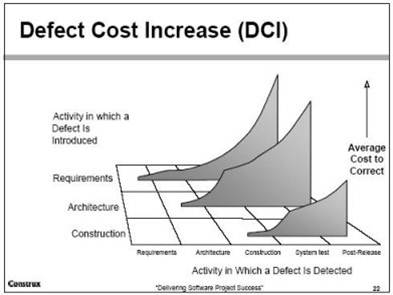
\includegraphics[width=0.75\linewidth]{defectcost.jpg} 
	\captionof{figure}{\cite{DefectPic}}
\end{Figure}

What we see here is that the earlier a defect is introduced the more it costs to fix it later. Of particular note is that the costs are roughly exponential, not linear. The longer a bug lies undetected, the increasingly harder it becomes to fix that bug. On the flip side, it's relatively easy to fix a bug that was introduced in the same stage that it is found, e.g. introducing a coding bug during ``Construction'' and fixing it while still writing code, prior to the ``System Test'' phase. 

% - CONSIDER REMOVING ALTOGETHER
% \subsubsection{Why Testing is Important}
% We're consistently surprised by how few people take testing seriously when it comes to non-trivial applications. Many developers will leave testing to their users, i.e., wait for users to have problems and report them before developers will fix them. This is an issue for a number of reasons, a few of which are: frustrated customers are unlikely to continue using a buggy product and are dissuaded from buying future products from the same developer, certain bugs can be security loopholes that may allow users access to information they shouldn't have, in the worst cases a bug may cause damage to a person or property and the developers would be on the hook.


%%%%%%%%%%%%%%%%%%%%%%
%%% Sample App 
%%%   Talk about test app
%%%%%%%%%%%%%%%%%%%%%%
\section{Sample App and Testing Frameworks}

\subsection{Sample ToDo App}
In order to test out the various frameworks that we found online, we needed a small application with some functionality, but without the inherent complexity that was going to come with our evaluation application. After some searching, We decided upon a Todo application made with Express.js, Node.js, and MongoDB. \cite{ToDoAppHomePage} Here is a brief preview of the app:

\begin{Figure}
  \centering
  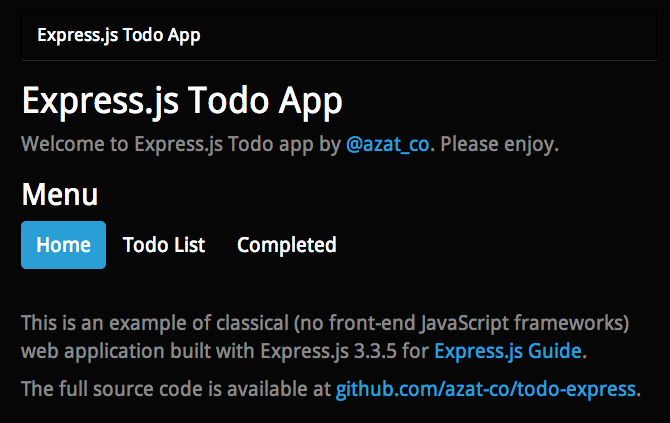
\includegraphics[width=0.75\linewidth]{todo_home.png}
  \captionof{figure}{ToDo app home page, simple three-button naviagation}
\end{Figure}

\begin{Figure}
  \centering
  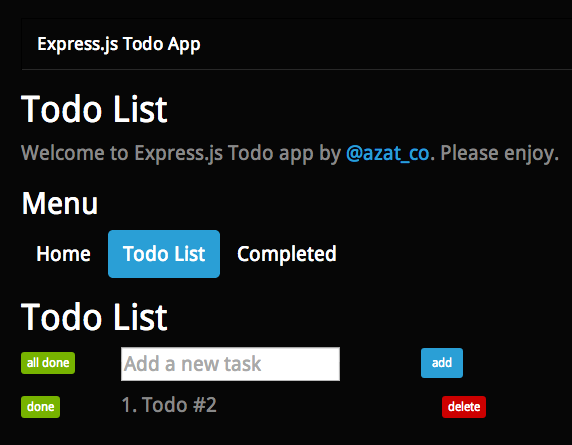
\includegraphics[width=0.75\linewidth]{todo_some_tasks.png}
  \captionof{figure}{ToDo app task page}
\end{Figure}

\begin{Figure}
  \centering
  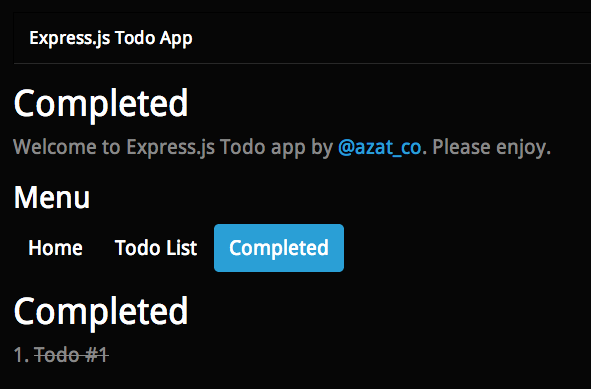
\includegraphics[width=0.75\linewidth]{todo_completed.png}
  \captionof{figure}{ToDo app completed tasks page}
\end{Figure}

This application was selected because it included Node.js and had enough functionality that tests wouldn't be completely trivial while also not being overwhelming.
One of the challenges in testing that we quickly came across was the asynchronous nature of the MongoDB calls that were made in the sample app. Because of this headache, we will be discussing how the following frameworks deal with asynchronous test support as JavaScript is inherently asynchronous.

%%%%%%%%%%%%%%%%%%%%%%
%%% Testing Frameworks
%%%   Talk about the various frameworks
%%%%%%%%%%%%%%%%%%%%%%
\section{Testing Frameworks}


% NOT SURE I NEED THIS SECTION AT ALL
% \subsection{Assumptions and Requirements}
% In order to more thoroughly vet the many testing frameworks we came across, we had a number of assumptions about the projects we'd be looking at and requirements for those framework. 
%- Node.js server because it's JS, so it's testable.
%- Something to do unit testing
%- Something to do continuous integration

\subsubsection{The Average Web Application}
In an effort to create a good workflow and collection of tools, we have chosen to focus on web applications that uses Node.js, Javascript, Cloud Services, and a backing Database when searching for our tools. This choice was made because of the popularity of that kind of set up, as well as the fact that our evaluation application was set up in that way.

\todo{THIS IS LAME}
Although there are multiple languages and tools available for creating a backing server, we chose Node.js because of it's wide use and because it is what we're most familiar with.

Javascript was chosen because it used in over 87\% of all websites. \cite{JSUsage} 

Many web applications use Cloud Services for a number of things, most often they're used for storage of the web content that's being hosted.

Web applications tend to keep track of users which most often constitutes the use of a database behind the scenes to store users and update them as necessary.

%- Node.js
%- Browser based
%- Javascript
%- Database
%- Open-source

\subsubsection{Tool Requirements}
\todo{Move this section elsewhere}
Our requirements for the selection of testing tools was relatively simple. In addition to meeting the requirements of our ``average web application'', the only other requirement was that the tool was free. What ``free'' means is that the developer would have access to at least the minimum functionality needed to use the tool on \emph{one} application that is \emph{open-source}. What we quickly found is that web testing tools love open-source projects but are far less willing to provide free functionality to private or closed-source projects. 

Occasionally the cost of tools will be discussed but in general we did not review tools that only offered paid options.
%- Free

\subsection{Unit Testing Frameworks}
The following frameworks are reviewed in chronological order of our evaluation. As such, comparisons will generally only be drawn between a framework and its predecessors in paper order. After all of the frameworks are outlined and evaluated, a longer section regarding the final decision will be made where comparisons will be drawn between all of them. 

An important distinction that needs to be made is that in web applications there is functionality behind the scenes and there is the UI element of the web page. Unit testing frameworks 

\subsubsection{Jasmine \cite{Jasmine}}
The first of the unit testing frameworks that we looked at was Jasmine, a Behavior Driven Development (BDD) testing framework. BDD is based on Test Driven Development and adds some simplifications and patterns that attempt to bring both developers and businessmen into the software testing process. The idea behind Behavior Driven Development is that input from non-technical stakeholders as well as technical stakeholders can come together so that everyone understands what the project should do.

This relates to Jasmine is the way that the developer writes Jasmine tests. The idea behind jasmine tests is that they read, as much as possible, like english sentences. As an example, the following is a valid Jasmine test:
\begin{lstlisting}
describe("Arithmetic Test", function () {
  it("should be able to compute the addition of two numbers", function () {
    expect(1 + 2).toEqual(3);
  });

  it("should be able to subtract numbers", function () {
    var theAnswer = 10;

    expect(12 - 2).toEqual(theAnswer);
  });
});
\end{lstlisting}
The ``describe'' statement creates a test suite to collect related tests under. Each ``it'' statement is generally one test with some number of ``expect'' statements. It may not be particularly pretty, but the above code is quite readable even to someone with no coding experience.

The default Jasmine package had some ineptitudes in dealing with Node.js but there was a package available through npm called jasmine-node \cite{JasmineNode} that gave jasmine access to the node package and functions. 

Asynchronous testing using Jasmine was a bit of a chore, but there is support built in. This support comes in the form of a three-set function progression. The first function, ``runs(function () \{ .... \})'', runs the asynchronous code. The second function, ``waitsFor(function () \{ ... \})'', polls a flag that is set by the first function when it completes. Finally, the third function, another ``runs(...)'', houses the assertions to determine if the code ran properly or not. This method requires a fairly substantial amount of typing as well as complicated function chains when more than one asynchronous call is required.

\subsubsection{Mocha \cite{Mocha}}
Mocha is another BDD testing framework that is almost identical to Jasmine. Unlike Jasmine, however, Mocha is not completely self-contained and requires an additional assertion library of one's choosing. We will outline our choice of Chai.js below.

Mocha also uses the ``describe -> it(\"should...\" '' patftern to create tests. There is no standard for writing expectation though, as each assertion library is likely to be slightly different.

Mocha's approach to asynchronous testing is quite a bit more straightforward than Jasmine's. In the ``it(...)'' anonymous function, there is passed an additional parameter called ``done'' which is then called when the asynchronous call has finished. This required us to edit the code we were testing to make all the async calls accept an additional callback, but it was a very small price to pay for extended testability. An example asynchronous test would look like this:
\begin{lstlisting}
describe("Asynch Mocha Test", function () {
  it("look like this", function (done) {
    myAsyncCall(param1, param2, function () {
      // This callback expected to run when async returns

      // Test ...
      // Test ...
      // ...
      done();
    });
  });
});
\end{lstlisting}

Overall Mocha offered more flexibilty at the cost of additional setup and better asynchronous support. This increased flexibility came in the way of being able to select our own assertion library so that our tests looked the way we wanted them. The cost of that was the need to find our own assertion library among the dozen that are out there. We prefer Mocha's method of asynchronous testing because it required considerably less typing on our part and was more easy to follow and read than a chain of method calls.

\paragraph{Assertion Library of Choice: Chai.js \cite{Chaijs}}
For the assertion library we chose Chai.js.  It offers the most flexibility for writing assertions that we'd found. It provides access to an Expect API, a Should API, and a more general Assert API. The Expect API provides assertions in the form of ``expect(myVar).to.equal(10);'' or ``expect(myArr).to.have.length(10);''. The Should API has assertions of the form ``myVar.should.be.a(\'number\');'' or ``myArr.should.have.length(10);''. Finally, the Assert API has the more tried and true ``assert.equal(myVar, 10);'' and ``assert.lengthOf(myArr, 10);''. The various APIs combined with Mocha's flexibilty led to a nice developer experience that can appeal to a variety of different developers.


\subsubsection{QUnit \cite{QUnit}}
QUnit is an Assertion style framework developed by the jQuery Foundation, the makers of jQuery, an immensely popular framework for DOM manipulation and access. QUnit is a bit more developer-centered and not as ``feel-good'' as the other frameworks but has, so far, been the most easy to use and has the most thorough test reporting of any framework out of the box. Mocha and Jasmine show how many ``specs'', the ``it'' functions, have passed, which is great information, but QUnit takes it a step further and breaks down each spec into the asserts contained within:
\begin{Figure}
  \centering
  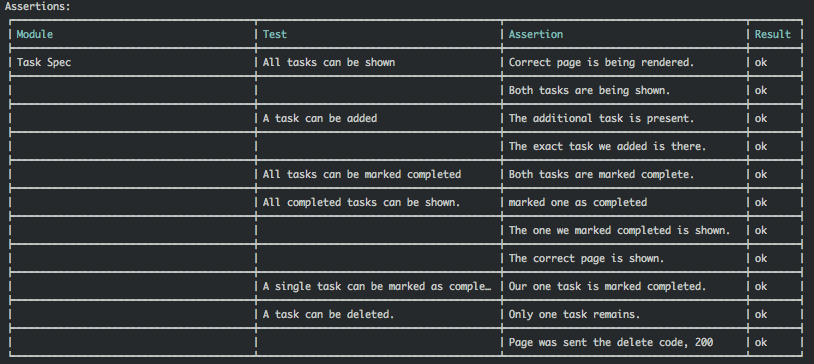
\includegraphics[width=\linewidth]{qunitrunner.png} 
  \captionof{figure}{Each individual spec is further broken down into the assertions within it.}
\end{Figure}
An interesting feature that QUnit has that we'd not seen elsewhere is the ability to specify how many assertions are expected to run in the test. This is incredibly useful for callbacks. By setting an expected number of assertions, tests can no longer fail silently just because an assertion was never run. If the QUnit test finishes and the assertion count is not what was specified, it will fail the test and let the developer know fewer assertions were called than expected.

QUnit isn't perfect however, QUnit tests are not grouped into suites by default and the syntax for grouping them leaves much to be desired. In order to group tests into ``modules'', as QUnit calls them, the developer writes code like the following:
\begin{lstlisting}
Qunit.module("Module A"); // All code following is grouped into Module A
test("Addition", function () {
  equal(2 + 2, 4, "Two + Two = Four");
  equal(3 + 5, 8, "Three + Five = Eight");
});
test("Subtraction", function () {
  equal(4 - 2, 2, "Four - Two = Two");
  equal(2 - 2, 0, "Two - Two = Zero");
});

// More tests....

QUnit.module("Module B");
// Tests under Module B

// ... Etc
\end{lstlisting}
It is difficult to visually see where one module starts and ends and so grouping and finding the right place to add a test can be a chore.

QUnit's handling of asynchronous tests is similar to Mocha's except instead of adding a parameter to the ``it'' function, the developer calls the ``asyncTest'' function instead. Finally, the developer calls ``start()'' when the asynchronous test is finished. Example:
\begin{lstlisting}
asyncTest("Async Test", function () {
  myAsyncCall(param1, param2, function () {
    // This callback expected to run when async returns

    // Test ...
    // Test ...
    // ...
    start();
  });
});
\end{lstlisting}

QUnit was a particularly strong contender when we saw the table that was produced after running the tests but its shortcomings led us to keep looking elsewhere. QUnit's handling of asynchronous tests is nice because they are more explicitly stated for the casual read-through instead of an extra parameter or set of functions within the test itself.

\subsubsection{Intern\cite{InternIO}}
Intern is a hybrid unit testing and browser testing framework that aims to be an all-in-one testing framework. Intern has unit testing, browser testing, and code coverage information all built into the same tool. Intern runs on its own server which give it access to the internals of the project, but caused problems when attempting to interact with a seperate server running the Node.js application. We were unable to get the browser testing portion of Intern to work because of the inability to set up cross-server communication easily and properly.

%- TDD, BDD, Object methods
Intern uses Chai.js for assertion methods but has it built-in as opposed to Mocha in which the developer had to get it themselves. This gives the developer access to Expect, Assert, and Intern's Object testing methods.

\todo{Add test code here!}

%- Integration with Selenium
Intern uses the WebDriver API to communicate with Selenium to drive the automated broswer testing portion of Intern. Selenium and the WebDriver API will be discussed in more detail in the next section ``Browser and UI Testing''.

%- Distinction between non-functional and functional tests
Intern's unit-test versus browser test seperation is termed, by Intern, nonfunctional versus functional testing. Nonfunctional tests are those that run without a browser while functional tests are WebDriver tests.

%- Code Coverage!
Intern includes configurable code coverage metrics on tests by default. Running unit tests gives the number of lines covered (ran) by the tests. Code coverage is provided by another Javascript library, Istanbul, created by Krishnan Anantheswaran \cite{Istanbul}.

Intern offered a one-stop shop for all of our testing needs but fell short when it came to configuring it for our Node.js server setup. If we had a more traditional web application setup with a seperate server that served normal HTML pages, Intern.io would have likely been our go-to tool for all of our testing needs.

\subsection{Browser and UI Testing}
Web applications, for the most part, require user input in order to be useful. The way the user interacts is through the outward facing web pages. Testing of a web application would be incomplete without testings the interactions and elements of these web pages. It's important that the inner workings are running the right code and producing the right answer, but it's almost just as important that the parameters get passed correctly and from the right places on the web pages. Also, it is important that navigation work as expected or a user will become frustrated and lose interest in the application.

What's important in browser testing is repeatability and being able to test on multiple browsers. Without the ability to automatically repeat tests, developers are left manually clicking through web pages every time anything changes. In addition, because there are so many different browsers and browser versions in the wild, it's important that the web pages run correctly (and predictably) on as many of them as possible.

% Browser Testing! Code
\subsubsection{Selenium\cite{Selenium}}
Selenium is an automated browser input runner. It is one of the only automated browser runners and certainly the most prominent. A developer can write code that will cause Selenium to drive a browser's input and assert expectations. On it's own Selenium has very minimal testing usage. It lacks a test reporting mechanism and only offers output in two forms: 1) No output at all, a browser window will open, input will be generated, and the window will close, or 2) the browser will exit with a cryptic error printed to the console. It is up to the developer to include print statements as to what is happening at any given time, what test is being run, and what the results are.

Generally, all browser testing tools will be using Selenium behind the scenes and doing the housekeeping automatically. This is the case for both of the web testing tools that will follow this description.

Selenium has support for running a number of different browsers. 

Having the ability to automatically run browser tests at any point takes a huge burden off of the web developer and allows for UI testing in addition to behind the scenes functionality testing. Whenever code is changed that may affect the UI flow or functionality, Selenium tests can be run withou the need for developers to manually click all of the HTML elements and input information in the relevant places.

Selenium's node incarnation is out-of-date and as such we had to change the selenium package to use the latest version of Selenium that works with the latest version of browsers. This required us to edit some of the javascript files that ran Selenium from the console using node. At the time of this writing, the Selenium node package was using Selenium 2.20 from over two years ago. The latest Selenium version is 2.40.

Selenium was written with maximum functionality and language flexability in mind and therefore can be incredibly verbose.

The Selenium WebDriver has APIs for a variety of programming languages including: Javascript, C, Java, and Python.

\subsubsection{Nightwatchjs\cite{NightwatchJS}}
Nightwatch is a Javascript testing library that wraps Selenium in an effort to make browser testing more concise and straightforward. Nightwatch uses Node.js' assertion library paired with Selenium's WebDriver to both run browser automation and also report test results.

Tests are written as a long chain of function calls that produce an easy-to-read series of browser events. For example, the following code segment opens a browser, goes to google.com, makes some assertions, writes ``nightwatch'' in the search box, clicks the search button, and then makes a few more assertions:
\begin{lstlisting}
module.exports = {
  "Demo test Google" : function (client) {
    client
      .url("http://www.google.com")
      .waitForElementVisible("body", 1000)
      .assert.title("Google")
      .assert.visible("input[type=text]")
      .setValue("input[type=text]", "nightwatch")
      .waitForElementVisible("button[name=btnG]", 1000)
      .click("button[name=btnG]")
      .pause(1000)
      .assert.containsText("#main", "The Night Watch")
      .end();
  }
};
\end{lstlisting}
As one can see, just reading the code line by line paints a picture of exactly what is happening and what is being checked for. 

The same code in normal Selenium is quite a bit more verbose:
\begin{lstlisting}
var assert = require('chai').assert,
    test = require('selenium-webdriver/testing'),
    webdriver = require('selenium-webdriver');

test.describe('Google Search', function() {
  test.it('should work', function() {
    var driver = new webdriver.Builder().
        withCapabilities(webdriver.Capabilities.chrome()).
        build();

    driver.get('http://www.google.com');
    driver.findElement(webdriver.By.name('q')).sendKeys('nightwatch');
    driver.findElement(webdriver.By.name('btnG')).click();

    driver.sleep(1000);
    driver.findElement(webdriver.By.id('main')).getText().then(function (text) {
        assert.isTrue(text.indexOf("The Night Watch") !== -1);
        driver.quit();
    });
  });
});
\end{lstlisting}

In addition to being more verbose, I've had to add an assertion library and this code has to be run using Node.js and the Mocha module instead of using the Selenium command.

Nightwatch is Node.js module, and as such can easily installed and run via npm and the command-line.

Though a small feature, Nightwatch has the ability to either assert or verify tests. The difference is that assertions will stop execution while verifications will merely log the failure and continue on. Verification can be useful if the developer wants to get an update on how many things are currently failing as opposed to having the entire test stop executing immediately after a single failure.

Nightwatch, as of this writing, has the ability to open Firefox, Chrome, and Internet Explorer. As of February 2014, Chrome is used by 46.69\% of internet users, Internet Explorer is used by 24.39\% and Firefox is used by 20.78\%.\cite{BrowserStats} Together that accounts for 91.86\% of all internet users.

\subsubsection{PhantomJS\cite{PhantomJS}}
% Too much.
%- Really great though, could be useful if needed.
%- Slow
%- FULL DOM/Browser emulation

\subsubsection{ZombieJS\cite{ZombieJS}}
%- Lightweight
%- Headless
%- NOT Full DOM emulation

\subsection{Continuous Integration Frameworks}
Continuous Integration frameworks attempt to make development easier by running specified actions, usually tests, after a change to the project. This change can be simply saving a modified file, or, more usually, an action like pushing a change to a repository.

Continuous Integration frameworks, therefore, need to be flexible in the type of project they support, customizable in their chosen environments to support differing projects, and have a simple way to connect to repositories or file systems.

\subsubsection{Jenkins \cite{Jenkins}}
Jenkins is the first of the continuous integration frameworks that we tried out. It was created by developers of a previous tool called Hudson when a dispute with Oracle led them to fork the Hudson project and rename it Jenkins. As of February 2014, the Jenkins organization has over 1,100 public repositories and 570 members. \cite{JenkinsGitHub} Jenkins has, according to their website, two main focuses: (1) building and testing software continuously and (2) monitoring executions of externally-run jobs. The first focus is the general goal for any CI framework. The second focus is of note and will be discussed after the initial evaluation. 

Jenkins is a series of web pages that are set up to run on a given server. This is what it looks like:
\begin{Figure}
  \centering
  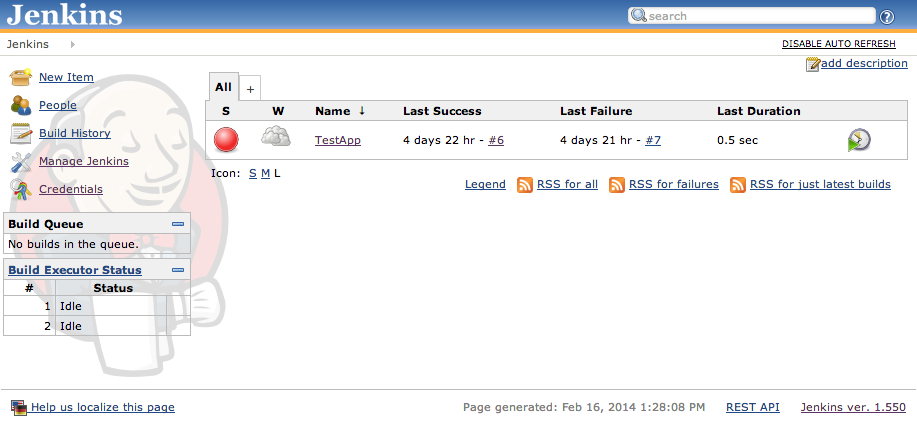
\includegraphics[width=0.95\linewidth]{jenkins.png}
\end{Figure}
Most companies give Jenkins a sub-domain on their web pages.

Jenkins comes bare-boned but is highly customizable and has a wide array of plugins. The plugins available integrate Jenkins with various services, integrate Jenkins with source control systems, and even just change the look of the Jenkins page or how it behaves. As an example, Jenkins can integrate with GitHub to run builds and tests when changes are pushed to a branch.

Because Jenkins comes bare and runs on the system of the devloper's choosing, it can run any project that is set up. The downside is that there is no support out-of-the-box unless the system already has the necessary compilers, interpreters, applications, and/or libraries installed.

One of the exceptional strengths of Jenkins is that the developer is only limited by the hardware of the machine running Jenkins. Any increase in computing power will be directly usable by Jenkins. Jenkins can run as many jobs as the server can handle at one time.

The other use for a tool like Jenkins is the ability to start services like cron jobs or similarly long-running tools and status monitors and then collect the output for them and allow the developer to check on them at any time.

Jenkins is an exceptionally strong tool for CI, but requires immense overhead in setting up the environment to run a project in. However, once the server has the necessary applications and libraries, the builds and tests will run without issue. Jenkins can run an ``unlimited'' number of builds, tests, and processes with the only limiting factor the hardware that it is running on. It is also 100\% free and can connect with public and private repositories alike.

\subsubsection{Travis \cite{Travis}}
Travis is an online continuous integration framework with 29 members and 64 repositories at the time of this writing. Unlike Jenkins, Travis is all online and includes a dashboard from which the developer can monitor builds and processes. Travis has a free version which is fully-featured but requires the project to be open-source and a paid version which gives the deveoper more processing power and access to private repositories.

Travis comes with internal support for eleven different languages including Node.JS, Ruby, Java, and Python. Travis has incredibly thorough documentation and a wealth of built-in services to work with projects if needed. Theses services include databases, notifications, deployment options, and GUI/Headless browsers. Travis supports all of the most popular databases: MySql, PostgreSql, MongoDB, CouchDB, and a myriad of others. It offers a number of notification options ranging from Email to IRC to HipChat (a chat service from Atlassian). Travis also offers deployment to just about every sort of provider there is, from Heroku to AWS S3 to RubyGems and also provides the ability to create custom web hooks to deploy to a provider not supported natively.

If at any point the project requires something that Travis does not support natively, Travis gives the permissions necessary to install any sort of libraries or services that can be installed with apt-get on an Ubuntu machine.

Travis requires that projects be hosted on GitHub, but by doing so the setup is incredibly easy. The developer signs into Travis using GitHub credentials and Travis pulls up all of the developer's repositories automatically. 

Getting a project running with Travis is fairly easy; just create a yml file in the repository with certain lines pertaining to the language, needed services, commands to run, etc. We were able to set up everything we needed in six simple lines.

In order to get access to private repositories, Travis offers several pricing plans, the cheapest of which is \$129 \cite{TravisPricing} for their ``Startup'' plan. That's a bit steep, but it does offer unlimited private repositories, unlimited collaborators, and two concurrent jobs. 

From what we gathered, Travis appears to be targeted at companies, not individual developers. Travis requires developers to host their projects on GitHub and only supports one process running at a time. However, Travis is incredibly easy to set up, does not require it's own server, comes with impressive built-in features, and works wonderfully with open-source repositories on GitHub.

\subsubsection{Semaphore \cite{Semaphore}}
Semaphore is another online CI framework that connects to GitHub to bring in projects. Semaphore is made by RenderedText, a software consulting team. Semaphore connects with public and private repositories but requires a subscription after 30 days no matter which repositories are used.

Semaphore was originally designed for only Ruby applications but in January of 2014 they announced official support for Node.js and Javascript and as of February 26th they now offer official support for Clojure projects.\cite{SemaphoreBlog} These types of projects require no setup or files in the repository, Semaphore automatically detects project type and auto-fills build steps. Their ``supported stack'' page also lists C/C++, Java, Perl, and Python, but those must be configured manually. 

Semaphore supports most databases and has a number of testing frameworks built-in. Once again any missing libraries or dependencies can be installed using apt-get. It would appear that deployment support is only available for Ruby projects.

Semaphore's pricing scheme is different than Travis' as it focuses on an individual, not a company. Their lowest cost subscription is one project (public or private) for \$14 per month. They offer more subscriptions with the ability to have more projects and concurrent processes in higher tiers.

Semaphore is still ruby-centric and requires a subscription. As our goal is to find a framework that is free for open-source projects, Semaphore was out automatically. It is included here because it's well-known and fairly established, especially in the ruby community.

\subsubsection{MagnumCI \cite{MagnumCI}}
MagnumCI is another online CI, it appears that Jenkins is one of the only ``off-line'' CI systems. MagnumCI has every feature available for free, however, it's still in public beta and although prices haven't been released, the team making MagnumCI has already stated that there will be price tiers. It is not unreasonable, though, to believe that MagnumCI will be free for open-source projects, and that's what we care about.

MagnumCI offers support for Ruby, PHP, Node.JS, and Go. MagnumCI, much like Semaphore, will attempt to auto-detect commands that it should run based on the project structure and language. All settings are overridable in a yml file.

MagnumCI has all the popular databases built-in, many of which run automatically on startup. MagnumCI also has two headless browser frameworks built in for running any browser testing that needs to be done. The developer can, again, use apt-get to install missing packages. MagnumCI does not, at current, provide automatic deployment options given a successful build.

Where MagnumCI shines is in support of different repositories. MagnumCI offers support for pulling from GitHub, BitBucket, GitLab, and a few others. It does require a bit more setup to get repositories connected, but what it comes down to is a couple lines of copied and pasted text within the repositories' settings.

Right now MagnumCI offers impressive features, private repositories, and extensive repository sources, all for free. It is hard to say that MagnumCI is the best because those features may end up costing money soon after this paper is completed. It is included in this review because it seems to be an up and comer that could prove quite strong.

\subsubsection{Drone.io \cite{DroneIO}}
Drone.io is an impressive online CI framework that offers substantial language support, is free for open-source projects, and offers the most reasonable pricing scheme for private repositories.

Drone.io supports eleven languages including: C++, Dart, Go, Haskell, Java, Node.JS, Ruby, and others. Setup requires the developer to specify language, as opposed to the automatic tools provided by the previous two CI frameworks, but will auto-generate built commands.

Drone.io offers support for most of the databases we've heard of, has a variety of deployment options, and is entirely configurable from the online dashboard. It also offers the most browsers and headless browsers for use with web page testing tools such as Selenium and PhantomJS.

Drone.io is able to connect to GitHub, BitBucket, and Google Code respositories to get projects automatically. Setup is simple, select the source of the repository (GitHub, BitBucket, or Google Code), select the repository from the list it gives once it connects, select the language of the repository, edit the default build script, and the project is ready to go.

Drone.io offers unlimited free open-source repositories. The next step up offers 5 private repositories for \$25 per month and for \$50 per month, unlimited private repositories. They also offer higher tier plans that allow for concurrently running builds.

Drone.io is a strong contender because of its language support, deployment options, and ease of setup. Where it lacks is in its notification options. The only notification option at present is email while other CI frameworks offer a number of other notification options for various messaging services.


\subsection{Misc Frameworks}
\subsubsection{Sauce Labs}


\subsubsection{Istanbul}


\subsubsection{Karma}

\subsubsection{Grunt.js}
- Task Runner
- Watch functionality
- Easy setup

\subsection{Misc Tools}
\subsubsection{Node Inspector}
Fantastic for debugging node.js server-side code!

%%%%%%%%%%%%%%%%%%%%%%
%%% Implementation 
%%%   Why we chose the tools we chose
%%%   Scripts written to help out 
%%%%%%%%%%%%%%%%%%%%%%
\section{Implementation}

\subsection{Chosen Toolset}
% - Unit Testing: Mocha w/ Chai
% - Coverage: Istanbul
% - CI: MagnumCI
% - Browser Testing: Nightwatch
% - Task Runner: Grunt
% - Package Manager: NPM, Bower


%%%%%%%%%%%%%%%%%%%%%%%%%
%%% Product 
%%% User Manual
%%%   Tools (programs, IDEs, scripts)
%%%   Setup instructions
%%%   Usage
%%%%%%%%%%%%%%%%%%%%%%%%%
\section{Product}

\subsection{Setup}

% - Note OS X 'ulimit' issue with Grunt-watch

\subsection{Workflow}
% - Unit Testing on save
% - CI used for running browser tests

% - 'Manually' instantiate Sauce Labs?


%%%%%%%%%%%%%%%%%%
%%% Evaluation
%%% PX Intro
%%%	Outline test suites
%%% PX Test metrics/results
%%%%%%%%%%%%%%%%%%
\section{Evaluation}

\subsection{PolyXpress (PX)}

\subsubsection{PolyXpress Author}
Our tests covered the Authoring portion of PX.

\subsection{Our Setup}
% - 15-inch MacBook Pro (Late 2008 model)
% -- Processor  2.53 GHz Intel Core 2 Duo
% -- Memory  4 GB 1067 MHz DDR3
% -- Graphics  NVIDIA GeForce 9400M 256 MB
% --- Not a particularly powerful computer, just your average everyday laptop.

% - OS 10.9.2
% -- Terminal
% - Sublime w/ plugins
% - Netbeans


%%%%%%%%%%%%%%%%%%%%
%%% Related Work 
%%% Similar testing frameworks
%%% 	Why they're not as good as ours
%%%%%%%%%%%%%%%%%%%%
\section{Related Work}
We were unable to find any works that attempted to bring existing technologies together to create a web testing framework. Instead, we came across a number of proprietary tools and research. Compared to these proprietary tools, the framework we already laid out is free and each part is supported by a community. There is no need to contact any paper authors to get software or support. We will, however, still outline them as they provided insight into what the problems in existing frameworks were, gaps in coverage, what was important in a framework, and inspiration and acknowledgment that this is a real problem that many people are trying to solve.

We also found research into common bugs, general testing techniques, and finding bugs that greatly improved our test cases and understanding.

\subsection{Testing Frameworks}

\subsubsection{``A Framework for Automated Testing of JavaScript Web Applications'' \cite{FrameworkForAutomatedTesting}}
A collection of IBM Researchers and two university students came up with a framework called ``Artemis'' for testing web applications. What is novel about their tool is that it generates test cases automatically based on execution patterns and feedback. They have attempted to solve the problem that writing test cases by hand is both time-consuming and often difficult. Their automatic test generation lead to an average of 69\% test coverage with enough tests generated.

Though it was an interesting and somewhat effective method, 69\% coverage is not great and this particular framework only covers the client-side, so it was incomplete for our purposes.

\subsubsection{``A Multi-Agent Software Environment for Testing Web-based Applications'' \cite{MultiAgentSoftwareEnvironment}}
Two students and a person from Lanware Limited brought AI into the web testing world with an agent-based environment for testing web applications. In order to split testing into manageable tasks for agents to carry out, they created an ontology for web testing using XML. Each agent is set up to handle one particular kind of testing with certain test data, i.e., a unit tester with data for one or two functions. This agent may then communicate with another agent who needs the results from that test, such as a test coverage agent or agent that is keeping track of test success and failure. This communication is done through a message-passing intermediary layer and a set of brokers who shuffle messages between agents.

This system is exciting and intricate but far too complex for a general web testing toolkit that just about any developer could pick up. It was important to weed techniques like this out as we wanted a fairly easy to use and understand toolkit.

\subsubsection{``A 2-Layer Model for the White-Box Testing of Web Applications'' \cite{2LayerModel}}
A couple of gentlemen at the Center for Scientific Research and Technology in Povo, Italy came with a model for white-box testing of web applications. (White box testing is when the developer is given access to the underlying code.) This paper breaks up the testing process into two abstraction levels, the navigation model, the way in which a webpage goes from page to page, and the control flow model, the way in which information is passed and stored on a given page or between pages. These constitute the 2-layers in the title. The navigation model represents high-level test cases, like asserting that a given link redirects to the correct location, while control flow represents low-level test cases, like making sure data is persisted between pages. 

This 2-layer approach is interesting and provided us with some insight, but the system was made for PHP applications and we weren't looking to implement a brand-new system and test PolyXpress with it all in one year.

\subsubsection{``Invariant-Based Automatic Testing of AJAX User Interfaces'' \cite{InvariantBasedUseInterfaces}}
Two individuals from the SOftware Engineering Research Group at Delft University in the Netherlands came up with a way to automatically test AJAX UI. The core of this idea is using a crawler to infer a flow graph. This paper outlines an plugin for an automated tool, ATUSA, for creating state validators and test suites for covering paths discovered during crawling (with a separate tool, CRAWLJAX). Their tests show that with minimal manual effort, the use of ATUSA can lead to high code coverage and error discovery. 

This tool showed promise as an AJAX testing tool, but we wanted something more generic. Their crawler, CRAWLJAX, however, was very interesting and while we didn't use it, the techniques it used are used in other tools we have.

\subsubsection{``JSART: JavaScript Assertion-based Regression Testing'' \cite{JSART}}
Two students from the University of British Columbia created a tool called JSART that uses run-time code instrumentation and analysis to infer invariants that can be used for regression testing. When the code runs, JSART creates a number of test cases that will be run the next time the code executes. The point being to catch any discrepancies between old code and new code. They ran their tool on nine web systems with fairly strong results. The tool was not perfect and occasionally created inappropriate tests, but generally the tests were appropriate and useful.

This is a useful concept that could be integrated into the toolkit at a later time.

\subsubsection{``DOM Transactions for Testing JavaScript'' \cite{DOMTransactions}}
Three people from Albert Ludwigs University in Germany came up with a way to deal with test fixtures that are built and torn down frequently. When testing JavaScript, many of one's tests will change the underlying web page in some way. This is often different from testing traditional software where components are separated. In order to test JavaScript, test fixtures for setting up the page and tearing down the page are exceptionally important. Because these fixtures are being made and torn down frequently, this paper discusses a way to utilize transactional memory to quickly get the web page into the right state without constant setup and tear down.

This could be integrated with one of the existing tools we will use, but our goal was to collect existing tools that did not need alteration.

\subsubsection{``Testing Web Applications in Practice'' \cite{TestingInPractice}}
Four students from the University of Seville, Spain published a paper with an overview of web testing. This paper was more of an introduction to testing, outlining the concepts of “Unit Testing”, “Integration Testing”, “Regression Testing”, testing the client versus testing the server, and a few others. It also describes how to test an actual web application using PHPUnit, a library similar to JUnit, for those developers familiar with Java. When writing their tests, they suggest taking more abstract actions and breaking them up into their functional parts and testing each of those. As an example, inserting a customer into the database (albeit not that abstract) is broken into tests for the function that inserts the customer and tests for making sure the customer makes it into the database.

The paper was good refresher on testing concepts and a hands-on application of those concepts. There wasn't any new information or tools to put toward our toolkit, but it was a good reminder and outlined some testing procedures.

\subsubsection{``Contract-Driven Testing of JavaScript Code'' \cite{ContractDrivenTesting}}
Two individuals from the Albert Ludwigs University in Germany created a tool, JSConTest, that provides a framework for making contracts for a JavaScript program, allowing for guided random testing on inputs and outputs. Contracts in JSConTest are comments above each function that are of the form ``type -> type''. More complicated forms can introduce parenthesis for function types. In general, JSConTest is useful for detecting type errors on input or output based on the operations performed within a function on the input and the result being output. 

Although JSConTest could be useful in a toolkit, its source is no-where to be found and there were other, more robust, tools out there for our purposes.

\subsubsection{``JAWS: A Javascript API for the Efficient Testing and Integration of Semantic Web Services'' \cite{JAWS}}
A researcher from Ford Motor Company published a paper regarding an API, called JAWS (Javascript, AJAX, Web Service), to facilitate testing and integration of Semantic Web Services. Semantic Web Services (SWS) are the server side of machine-to-machine interaction via the internet. This is opposed to machine-to-human interaction such as web pages that one visits personally. SWS use markup that is detailed and sophisticated which conforms to certain standards but is not human-readable.

Another interesting API and project, but we are not focusing on SWS and so including a tool or API like JAWS would be overkill and beyond trying to keep the toolkit as simple and robust as possible.

\subsubsection{``WebMate: A Tool for Testing Web 2.0 Applications'' \cite{WebMate}}
Four people from Saarland University in Germany created a tool, WebMate, for automatically navigating web-pages with dynamic content and data. WebMate's goal is to output a usage model for testing purposes. This usage model allows tests to be focused on navigation as well as functionality. This dual usage leads to the ability to test the experience as well as the functions. In addition, WebMate can be used for Cross-Browser testing by running it on multiple browsers and comparing the results. In essence, WebMate is a web application crawler seeking to automatically suss out the layout and interaction between web pages to provide a model to the tester, be it a developer or the automatic testing capabilities of WebMate.

WebMate was another interesting project that could have seen use in our toolkit if crawlers weren't already available in other, more mainstream, tools.

\subsubsection{``Continuous Testing with Ruby, Rails, and JavaScript'' \cite{BookContinuousTesting}}
The well known book by Rady and Coffin talks about Continuous Testing and has lots of examples. The last two chapters of the book, six and seven, talk about setting up a Continuous Testing environment for JavaScript using Node.js and a number of other tools. It fit almost perfectly with our project and was used as the basis of our testing setup. They use JSLint for linting, Jasmine for test cases, and Watchr for running the tests continuously. Lastly it discussed writing effective tests, which is always important.

Not all of those tools made it into the eventual final toolkit, but they were all important to look at in the context of making the overarching toolkit.

\subsection{Finding Bugs}
One of the most important aspects of testing is actually finding the bugs in the program. A number of sources provided guidelines and suggestions for finding bugs in web applications.

\subsubsection{``Finding Bugs In Dynamic Web Applications'' \cite{FindingBugs}}
Seven researchers from the MIT Computer Science and Artificial Intelligence Lab wrote a paper addressing testing in dynamic web applications. Common testing techniques were not made to work with dynamic content that can be generated at the drop of a hat or click of a button. Therefore, common testing techniques are inadequate for testing dynamic web applications. This paper discusses ways to find bugs in these new-fangled dynamic web applications. They use a new technique and extended a tool called Apollo. This technique generates dynamic test cases based on concrete and symbolic execution. ``The basic idea is to execute an application on an initial input (e.g., an unconstrained or randomly chosen input), and then on additional inputs obtained by solving constraints derived from exercised control flow paths.''

Although they test PHP applications, the extension to JavaScript is fairly straightforward. We didn't use Apollo, but the techniques described within allowed for more focused and productive testing.

\subsubsection{``Testing Web Services: A Survey'' \cite{TestingWebServicesSurvey}}
Three researchers at the Centre for Research on Evolution, Search \& Testing at King's College in London wrote a survey of web frameworks for testing web services. Their focus is on Service-Oriented Computing, a paradigm in which web sites or applications provide small pieces of functionality usable by ``anyone''. These services are then combined to create more fully featured applications. What they note in particular is that when using web services, the developer rarely has access to the source code and must therefore black-box test them. Corollary to that is that the developer has to implicitly trust whoever made the service. They go through and discuss a number of frameworks and come to the conclusion that it's most certainly not a solved problem for the following reasons: The frequency of testing required, Testing without disrupting the operation of the service, Determining when testing is required and which operations need to be tested. Regarding the frequency of testing, web services often change in effort to make improvements, but those improvements can change the services and break tests. Testing without disrupting service is difficult because these services often limit accesses or simultaneous access of both a test and a running web application. Finally, determining when and what to test comes back to the trust issue. Some services provide their own testing metrics that include code coverage, number of tests, etc, but the developer must trust that the service is thoroughly tested, not just tested enough to provide interesting metrics.

\subsubsection{``A Framework for Testing RESTful Web Services'' \cite{RESTfulFramework}}
Two people from the University of Dakota School of Aerospace Studies outline a framework for testing RESTful web services. RESTful web services, short for Representation State Transfer, are, in the context of web applications, a name for web APIs that conform to a set of constraints. In particular they must offer four request methods: GET, POST, PUT, and DELETE. These methods generally connect to a database or other storage system in order to store, retrieve, or delete entries therein.

\todo{Finish reading this paper... My bad Dr. Haungs.}

\subsection{Writing Effective Test Cases}
Although not too distinct from \emph{finding bugs}, writing effective test cases is its own art form. The important of writing concise, correct, productive test cases cannot be overstated. The difference between writing one test case that effective tests multiple things and writing a single test case for every little detail is the difference between developers wanting to write tests at all and skipping it due to time constraints or frustration.

\subsubsection{``Going Faster: Testing The Web Application'' \cite{GoingFaster}}
Two employees of Evant Software wrote an article for IEEE Software regarding the testing of web applications. Mostly this paper was an overview and implementation of Test Driven Development (TDD) and eXtreme Programming, but in the middle of the article was a good section about the difficulties of testing the web and how to deal them. A few of the remarks regarding the difficulty of web testing is that often the client-side and server-side portions of web applications are written in different languages. This wasn't an issue for our application, but is still an issue for many applications. Some of the most useful advice was: ``First, test those parts of the server-side code that are not directly concerned with being part of the Web application, without involving Web peculiarities. ... Second, test those parts of the client-side code that have no server interaction. This is typically code that contains little or no business logic. ... Third, write functional tests of a low grain in the server-side language (for example, Java or C++) that simulate the request/response Web environment. ... Using this framework you can write walk-through tests that simulate the user moving through the UI''.

This step-by-step walkthrough of how to test was an excellent starting point to look at different tools and how they handled this issue.

%%%%%%%%%%%%%%%%%%
%%% Conclusion 
%%% Summary of what they just read
%%% Recap results
%%%%%%%%%%%%%%%%%%
\section{Conclusion}


%%%%%%%%%%%%%%%%%%%
%%% Future Work 
%%% Anything we wanted to do but didn't have time to
%%%%%%%%%%%%%%%%%%%
\section{Future Work}

% -- Extension to all of PX?
% -- Extension to non-proprietary open-source project


%%%%%%%%%%%%%%%%%
%%% Appendices
%%% Actual Test Code
%%% Anything that needs an appendix
%%%%%%%%%%%%%%%%%
\section{Appendices}

\subsection{ToDo App Test Code}

\subsection{PolyXpress Test Code}

% \end{multicols}
\newpage

\bibliographystyle{IEEEannot}

\bibliography{paper}

\nocite{*}

\end{document}
